\section{Решение} 


\subsection{Установка и настройка LSF}

Настройка значений полей в конфиг-файле \lstinline{install.config} \cite{install_plan}:
\begin{lstlisting}
LSF_ADMINS="lsfadmin"
LSF_TOP="/usr/share/lsf"
LSF_ADD_SERVERS="hostm hostb hostc hostd"
LSF_MASTER_LIST="hostm hostd"
LSF_ADD_CLIENTS="hoste hostf"
LSF_CLUSTER_NAME="cluster1"
CONFIGURATION_TEMPLATE="HIGH_THROUGHPUT"    
\end{lstlisting}

Пояснение полей:

\lstinline{LSF_ADMINS}: имена пользователей администраторов LSF;

\lstinline{LSF_TOP}: полный путь директории установки LSF;

\lstinline{LSF_ADD_SERVERS}: узлы, которые могут ставить задания в очередь и выполнять задания;

\lstinline{LSF_MASTER_LIST}: узел сервера LSF, который действует как всеобщий координатор для кластера. В каждом кластере есть один главный узел, который выполняет планирование и отправку всех заданий из очереди в узлы для выполнения;

\lstinline{LSF_ADD_CLIENTS}: узлы, которые могут только ставить задания в очередь;

\lstinline{LSF_CLUSTER_NAME}: имя кластера LSF;

\lstinline{CONFIGURATION_TEMPLATE}: шаблон конфигурации для определения начальной конфигурации нового кластера \cite{lsf_overview,host_types_models}.

Создание пользователя для администратора LSF и запуск установки LSF: 
\begin{lstlisting}
$ sudo -i
# adduser lsfadmin
# ./lsfinstall -f install.config
\end{lstlisting}

Запуск LSF:
\begin{lstlisting}
# source /usr/share/lsf/conf/profile.lsf
# lsfstartup
\end{lstlisting}

Настройка автозапуска LSF:
\begin{lstlisting}
# cd /usr/share/lsf/10.1/install
# ./hostsetup --top="/usr/share/lsf" --boot="y"
\end{lstlisting}


\subsection{Поддержка API для LSF в серверной части Scheduler}

Shell-скрипты формируют файл c информацией для запуска задачи, который запускается командой \lstinline{bsub} - она считывает файл задачи, параметры в виде строк начинающихся с \lstinline{#BSUB} и запрашивает в системе очередей необходимые ресурсы, после чего задача ставится в очередь и, когда запрошенные ресурсы освобождаются, исполняется остальная часть. \lstinline{job_file} - это shell-скрипт с прописанными директивами \lstinline{#BSUB} в начале файла.

За основу взяты шаблоны задач и скрипты bash системы очередей Torque для поддержки LSF. Шаблоны задач и скрипты Torque переписаны для LSF. Созданы shell скрипты, которые формируют файл c информацией для запуска задачи

\lstinline{run_rnkim_decomp_mpi_lsf.sh},

\lstinline{run_rnkim_mpi_lsf.sh},

\lstinline{run_rnkim_omp_lsf.sh}

и шаблоны задач

\lstinline{template_rnkim_decomp_lsf},

\lstinline{template_rnkim_decomp_mpi_lsf},

\lstinline{template_rnkim_mpi_lsf},

\lstinline{template_rnkim_omp_lsf}

для LSF.

Переписывание скриптов bash с Torque на LSF:

{
\lstset{emph={job_file}, emphstyle=\itshape}
Отправка задачи \lstinline{job_file} в очередь 

\begin{lstlisting}
qsub job_file
-->
bsub < job_file
\end{lstlisting}
}

В параметр \lstinline{-m} --- конкретные хосты, группы хостов, вычислительные единицы --- передаются теги или типы узлов.

\begin{lstlisting}
$NODETYPE
-->
_tmplNODETYPE_="#BSUB -m \"$NODETYPE\""
\end{lstlisting}

Переписывание шаблонов задач с Torque на LSF:

В параметр \lstinline{-n} --- задает кол-во тасков в задаче --- передается кол-во ядер в узле \lstinline{_tmplCORES_}.

В параметр \lstinline{-R} --- задает строку ресурсов --- передается кол-во узлов \lstinline{1} \cite{ref_bsub}.
\begin{lstlisting}
#PBS -l nodes=1_tmplNODETYPE_:ppn=_tmplCORES_
-->
#BSUB -n _tmplCORES_ -R "span[hosts=1]"
_tmplNODETYPE_
\end{lstlisting}

В параметр \lstinline{-n} --- задает кол-во тасков в задаче --- передается кол-во всех ядер в узлах \lstinline{_tmplTOTALCORES_}.

В параметр \lstinline{-R} --- задает строку ресурсов --- передается кол-во ядер на узел \lstinline{_tmplCORES_}.
\begin{lstlisting}
#PBS -l nodes=_tmplNNODES__tmplNODETYPE_:ppn=_tmplCORES_
-->
#BSUB -n _tmplTOTALCORES_ -R "span[ptile=_tmplCORES_]"
_tmplNODETYPE_

TOTALCORES = NNODES * CORES
\end{lstlisting}

В параметр \lstinline{-notify} --- запрашивает уведомление пользователя, когда задание достигает любого из указанных состояний --- передаются состояния программы.

В параметр \lstinline{-R} --- отправляет письмо по указанному адресу электронной почты --- передается адрес электронной почты.
\begin{lstlisting}
#PBS -m ea
#PBS -M <usermail>
-->
#BSUB -notify "exit done"
#BSUB -u <usermail>
\end{lstlisting}

В параметр \lstinline{-R} --- присваивает указанное имя заданию --- передается имя модели.

В параметр \lstinline{-W} --- устанавливает ограничение времени выполнения задания --- передается период 150 часов.

В параметр \lstinline{-cwd} --- задает текущую рабочую директорию для выполнения задания --- передается путь директории.
\begin{lstlisting}
#PBS -N _tmplMODEL_
#PBS -l walltime=150:00:00
#PBS -d _tmplDIR_
-->
#BSUB -J _tmplMODEL_
#BSUB -W 150:00
#BSUB -cwd _tmplDIR_
\end{lstlisting}


\subsection{Поддержка команд, направляемы напрямую из Scheduler на кластер}

Команды в Scheduler, относящиеся к конкретной системе очередей, хранятся в значениях ключей в словаре (тип данных на Python). Значениям соответствуют либо ссылки на исполняемые на сервере скрипты, либо команды для системы очередей, либо ссылки на методы обработки. Для LSF добавлены следующие значения:
\begin{lstlisting}
%Ключ%:                    %Значение%
QsysCMD.RUN_OMP:         "$RNKIMPATH/scripts/run_rnkim_omp_lsf.sh",
QsysCMD.RUN_MPI:         "$RNKIMPATH/scripts/run_rnkim_decomp_mpi_lsf.sh",
QsysCMD.RUN_MPI_ADV:     "$RNKIMPATH/scripts/run_rnkim_mpi_lsf.sh",
QsysCMD.DEL_TASK:        "bkill",
QsysCMD.GET_STAT:        "bjobs -json -o 'jobid user stat job_name submit_time start_time finish_time error_file output_file effective_resreq slots'",
QsysCMD.GET_STAT_MTHD:   lambda str_jobs: f"bjobs -json -o 'jobid user stat job_name submit_time start_time finish_time error_file output_file effective_resreq slots' {str_jobs}",
QsysCMD.PARSE_ID_MTHD:   lambda strout: int(strout[strout.find('<') + 1:strout.find('>')]),
QsysCMD.UPDT_JSTAT_MTHD: self._update_jstats_lsf
\end{lstlisting}

Метод \lstinline{_update_jstats_lsf} обновляет статус моделей. Парсит JSON статуса модели и вызывает метод \lstinline{_pars_job_json_lsf} для парсинга значений полей JSON статуса.

Метод \lstinline{_update_jstats_lsf} парсит поля с значениями у JSON статуса и записывает ключ 'имя модели' со значением словарь состояния:
\begin{lstlisting}
{
    "JOBID":"1363",
    "USER":"vagrant",
    "STAT":"EXIT",
    "JOB_NAME":"MODEL.DATA",
    "SUBMIT_TIME":"Jun  7 08:19",
    "START_TIME":"Jun  7 08:19",
    "FINISH_TIME":"Jun  7 08:19 L",
    "ERROR_FILE":"",
    "OUTPUT_FILE":"",
    "EFFECTIVE_RESREQ":"select[type == local] order[r15s:pg] span[ptile=2] ",
    "SLOTS":"2"
}
-->
model_name:
    {
        JobStat.ACC_NAME: str,
        JobStat.JOB_NAME: str,
        JobStat.OUT_PATH: str,
        JobStat.ERR_PATH: str,
        JobStat.JOB_STAT: ModelState,
        JobStat.NUM_NODES: int,
        JobStat.QUEUE_TIME: datetime,
        JobStat.START_TIME: datetime,
        JobStat.COMPL_TIME: datetime
    }
\end{lstlisting}


\subsection{Тестирование}

Использован программный продукт виртуализации VirtualBox для тестирования. Сервер установлен на виртуальной машине VirtualBox с операционной системой Ubuntu Server 18.04. Клиент запускался в исходной машине и связывался с виртуальной машиной с сервером.

\begin{figure}[h]
    \centering
    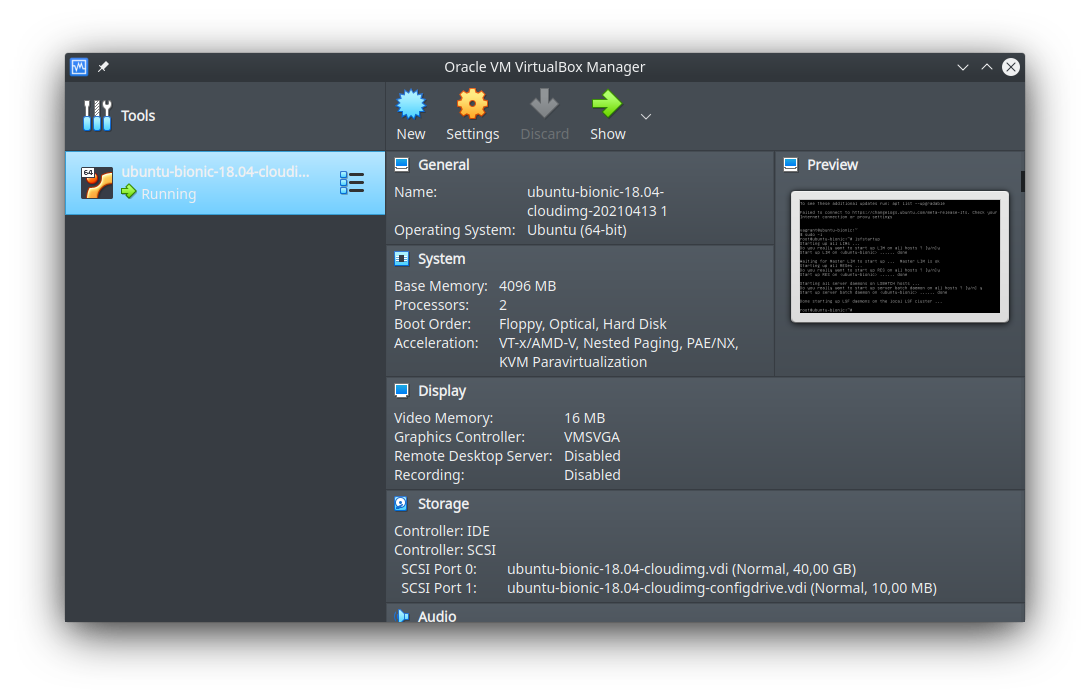
\includegraphics[width=\linewidth]{vbox.png}
    \caption{VirtualBox}
    % \label{fig:block-scheme}
\end{figure}

\begin{figure}[h]
    \centering
    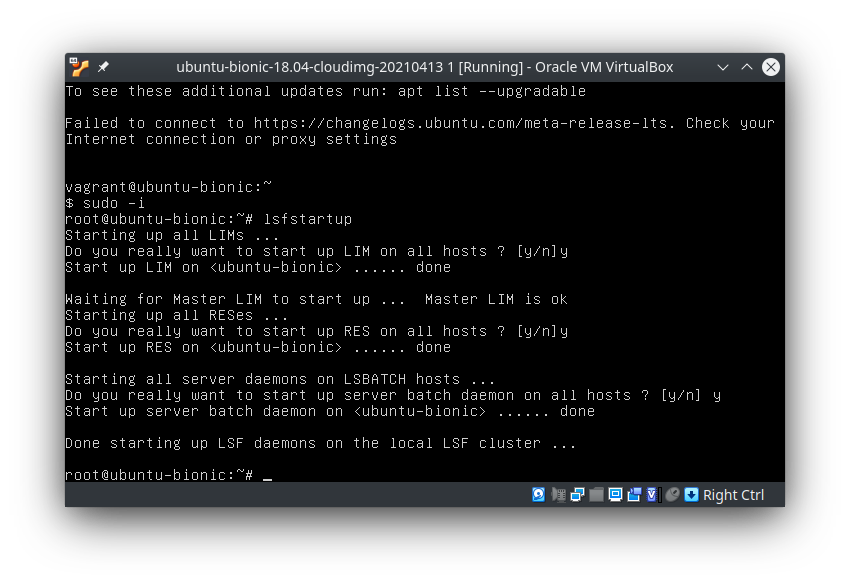
\includegraphics[width=\linewidth]{vm.png}
    \caption{Виртуальная машина. Изображен запуск LSF}
    % \label{fig:block-scheme}
\end{figure}

\begin{figure}[h]
    \centering
    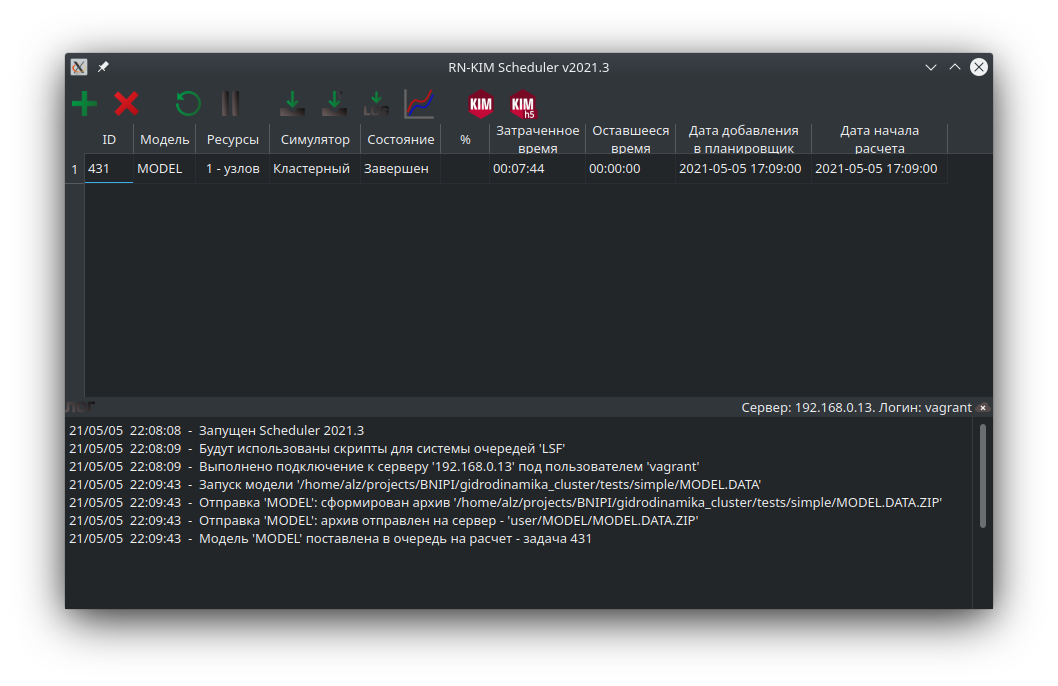
\includegraphics[width=\linewidth]{type_cluster.png}
    \caption{Скриншот Scheduler. Тип расчета модели: кластерный}
    % \label{fig:block-scheme}
\end{figure}

\begin{figure}[h]
    \centering
    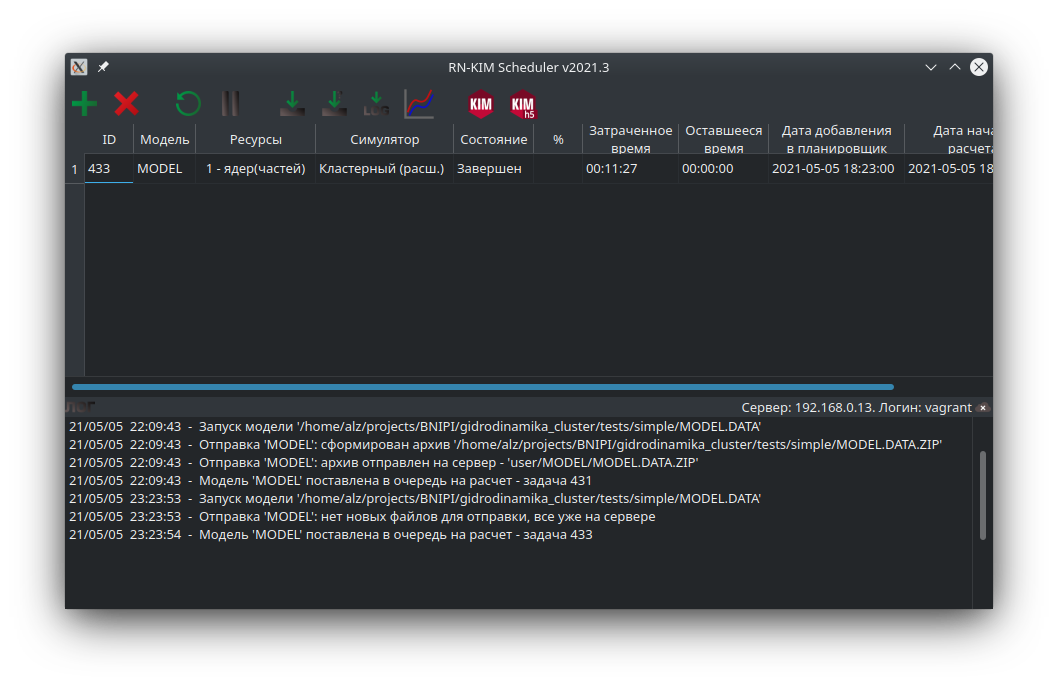
\includegraphics[width=\linewidth]{type_cluster_expanded.png}
    \caption{Скриншот Scheduler. Тип расчета модели: кластерный (расш.)}
    % \label{fig:block-scheme}
\end{figure}

\begin{figure}[h]
    \centering
    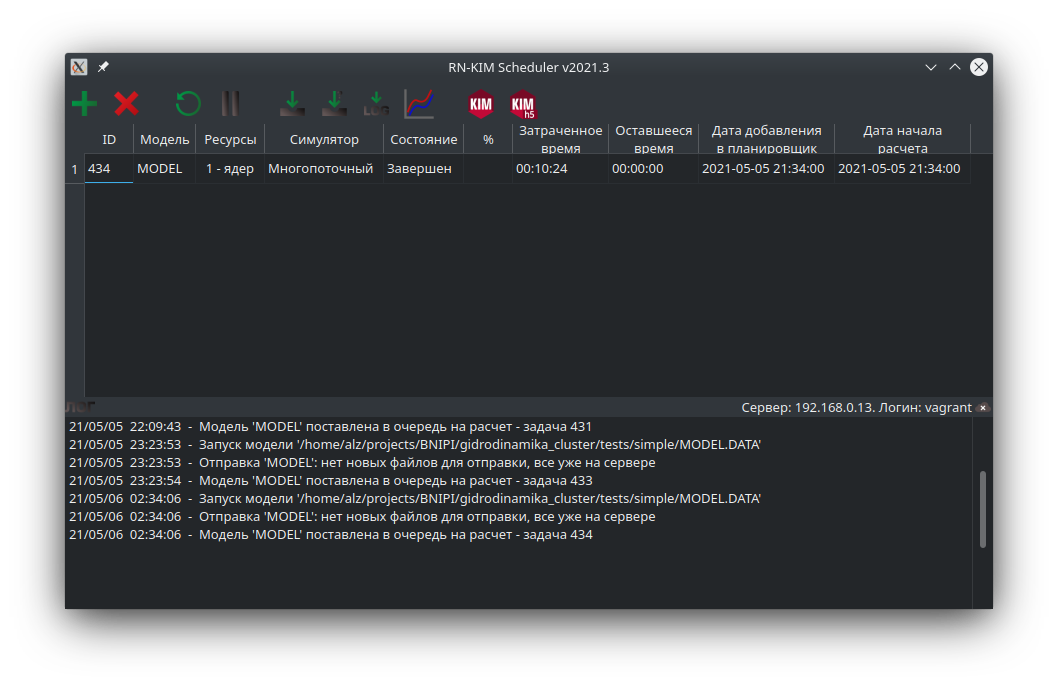
\includegraphics[width=\linewidth]{type_multithread.png}
    \caption{Скриншот Scheduler. Тип расчета модели: многопоточный}
    % \label{fig:block-scheme}
\end{figure}

\begin{figure}[h]
    \centering
    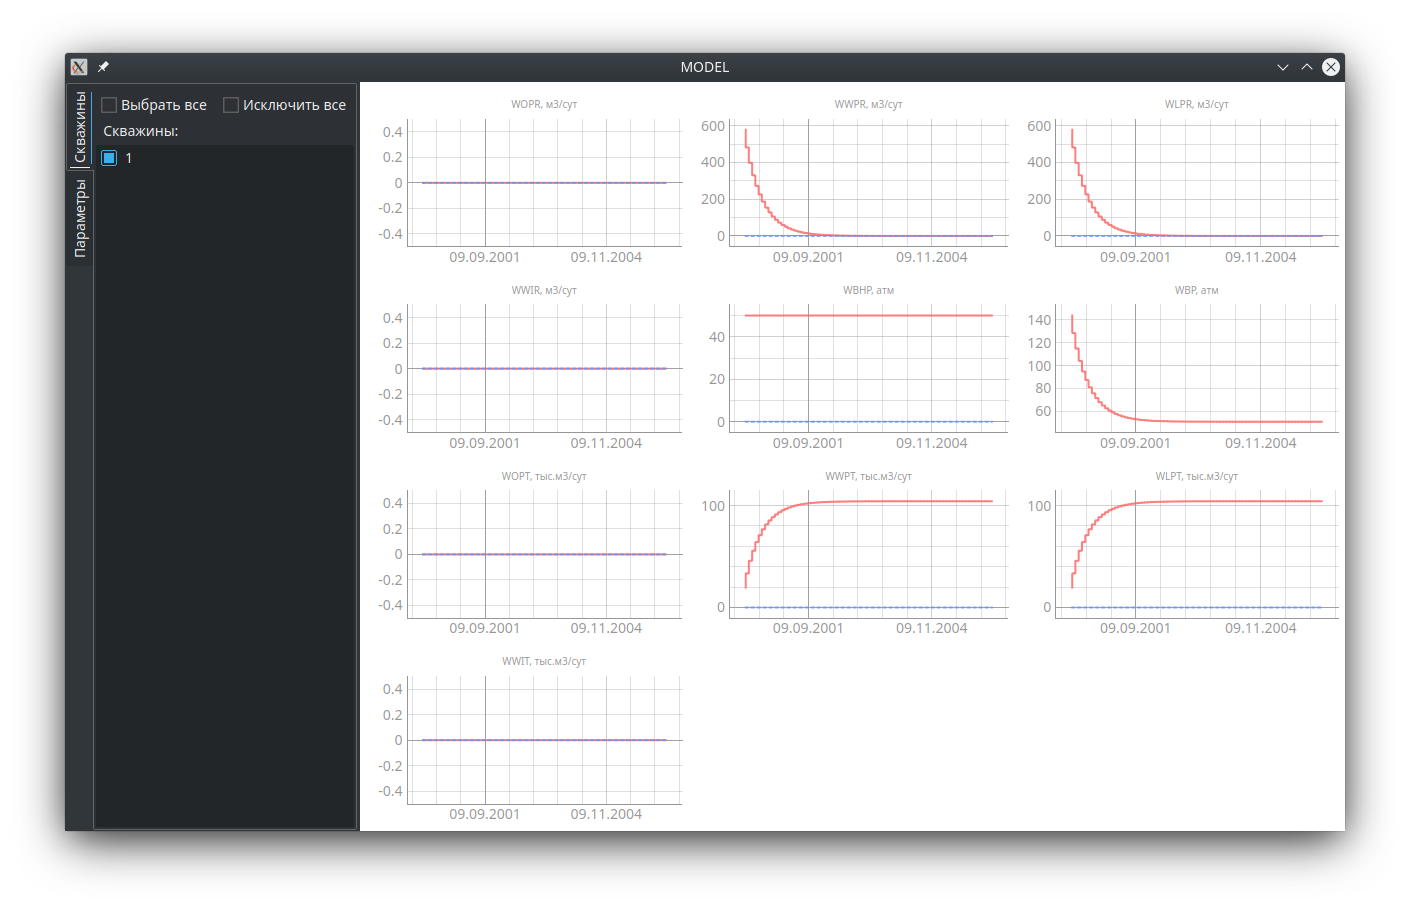
\includegraphics[width=\linewidth]{curves.png}
    \caption{Скриншот Scheduler. Рассчитанные кривые модели}
    % \label{fig:block-scheme}
\end{figure}

\clearpage